\begin{frame}[fragile]

  {\Huge Batched BLAS and LAPACK}

  \vspace{20pt}

  \textbf{Learning objectives:}
  \begin{itemize}
    \item {Motivation for batched functions}
    \item {Two namespaces with BLAS and LAPACK functions}
    \item {Calling batched functions}
  \end{itemize}

  \vspace{-20pt}

\end{frame}

%==========================================================================
% Slide 11
\begin{frame}[fragile]{Parallel Batched BLAS/LAPACK Interface}

Batched BLAS/LAPACK is {\bf simple} i.e., BLAS/LAPACK in a parallel loop

  \begin{code}[frame=single, keywords={}, backgroundcolor=\color{brown!10}, basicstyle=\tiny]
auto A = Kokkos::View<double***>(''A'', N, Blk, Blk);
Kokkos::parallel_for( RangePolicy(N), /// users' parallel execution policy
  KOKKOS_LAMBDA(int &i) {
  auto AA = Kokkos::subview(A, i, ALL, ALL);
  KokkosBatched::SerialLU(AA);  /// functor-level interface
});
  \end{code}
\vspace{1pt}
Kokkos batched BLAS/LAPACK is made up of following two components
\begin{itemize}
\item Kokkos parallel execution policy with \verb|parallel_for|
\item A functor-level interface to be used in \verb|operator()|
\end{itemize}
\vspace{1pt}
Hierarchical functor interface is required matching to Kokkos' hierarchical parallelism

\end{frame}
  
\begin{frame}[fragile]{Layered Hierarchical Functor-level Interface}

  {\bf Serial Interface}
  \begin{itemize}
  \item \small{can be used in a flat \verb|parallel_for| i.e., \verb|Kokkos::RangePolicy|}
  \item \small{can be used in the most inner loop of nested \verb|parallel_for|'s}
  \end{itemize}
  \begin{columns}[t,onlytextwidth]
    \column{.475\textwidth}
  \textbf{\tiny{Serial with RangePolicy}}
  \begin{code}[frame=single, keywords={}, backgroundcolor=\color{brown!10}, basicstyle=\tiny, breaklines=true]
parallel_for(RangePolicy, 
 KOKKOS_LAMBDA(int &idx){
   KokkosBatched::SerialDoThing();
}); 
  \end{code}

    \column{.05\textwidth}
    \column{.475\textwidth}
  \textbf{\tiny{Serial in Hierarchical parallel loops}}
  \begin{code}[frame=single, keywords={}, backgroundcolor=\color{brown!10}, basicstyle=\tiny, breaklines=true]
parallel_for(TeamPolicy,
 KOKKOS_LAMBDA(member_type &member){
   parallel_for(TeamThreadRange) {
     parallel_for(ThreadVectorRange) {
       KokkosBatched::SerialDoSomething();
}); }); }); 
  \end{code}
  \end{columns}
\end{frame}

\begin{frame}[fragile]{Layered Hierarchical Functor-level Interface}

  {\bf TeamVector Interface}
  \begin{itemize}
  \item \small{internally uses two nested \verb|parallel_for| with \verb|TeamThreadRange| and \verb|ThreadVectorRange|}
  \item \small{requires the member (thread communicator) as an input argument}
  \end{itemize}
  \textbf{\tiny{TeamVector with TeamPolicy}}
  \begin{code}[frame=single, keywords={}, backgroundcolor=\color{brown!10}, basicstyle=\tiny, breaklines=true]
parallel_for(TeamPolicy, 
 KOKKOS_LAMBDA(member_type &member){
   KokkosBatched::TeamVectorDoSomething(member);
}); 
  \end{code}
\end{frame}

\begin{frame}[fragile]{Layered Hierarchical Functor-level Interface}

  {\bf Team Interface}
  \begin{itemize}
  \item \small{internally use \verb|TeamThreadRange| only}
  \item \small{in general is used with SIMD or Ensemble types where vector parallelism is expressed within the type}
  \item \small{can include \verb|ThreadVectorRange|}
  \end{itemize}
  \begin{columns}[t,onlytextwidth]
    \column{.475\textwidth}
  \textbf{\tiny{Team without ThreadVectorRange}}
  \begin{code}[frame=single, keywords={}, backgroundcolor=\color{brown!10}, basicstyle=\tiny, breaklines=true]
parallel_for(TeamPolicy, 
  KOKKOS_LAMBDA(member_type &member){
  KokkosBatched::TeamDoThing(member);
}); 
  \end{code}

    \column{.05\textwidth}
    \column{.475\textwidth}
  \textbf{\tiny{Team with ThreadVectorRange outside}}
  \begin{code}[frame=single, keywords={}, backgroundcolor=\color{brown!10}, basicstyle=\tiny, breaklines=true]
parallel_for(TeamPolicy,
 KOKKOS_LAMBDA(member_type &member){
   parallel_for(ThreadVectorRange) {
     KokkosBatched::TeamDoSomething(member);
}); }); 
  \end{code}
  \end{columns}
\end{frame}

%==========================================================================
\begin{frame}[fragile]{User Composable Batched BLAS and LAPACK}

  \textbf{} \\
  \vspace{26pt}
  Consider a batched \textbf{block matrix inversion} which can be used for a block
  Jacobi solver. \\
\end{frame}

%==========================================================================
\begin{frame}[fragile]{User Composable Batched BLAS and LAPACK}

  \textbf{KokkosKernels} \\
  \vspace{10pt}
  %\begin{tabular}{|p{3.6cm}|p{3.6cm}|}
  %  KokkosKernels  &  Vendor Libraries \\
    \begin{code}[keywords={parallel_for,auto,const,double}]
      using ViewTypeAs = Kokkos::View<double***>;


      using ScratchSpaceView = Kokkos::View<double*,
        Kokkos::DefaultExecutionSpace::scratch_memory_space,
        Kokkos::MemoryTraits<Kokkos::Unmanaged>>;
    \end{code}
  \end{frame}
  \begin{frame}[fragile]{User Composable Batched BLAS and LAPACK}

  \textbf{KokkosKernels} \\
    \begin{code}[keywords={parallel_for,auto,const,double}]
      ViewTypeAs As("As", N, Blk, Blk);
      Kokkos::parallel_for(TeamPolicy,
        KOKKOS_LAMBDA(member_type &member) {
          auto A = Kokkos::subview(As, i, ALL, ALL);
          auto T = ScratchSpaceView(member, Blk, Blk);
          KokkosBatched::TeamVectorLU(member, A);
          KokkosBatched::TeamVectorCopy(member, T, A);
          KokkosBatched::TeamVectorSetIdentity(member, A);
          KokkosBatched::TeamVectorLowerTrsm(member, T, A);
          KokkosBatched::TeamVectorUpperTrsm(member, T, A);
      });
    \end{code}
    \begin{itemize}
      \item \small{Multiple BLAS/LAPACK operations can be fused in a single kernel}
      \item \small{Temporal locality via single kernel launch}
      \item \small{Local cache memory can be used as scratch space}
      \item \small{Team size can be tuned for problem}
      \item \small{Poor performance when poorly tuned}
    \end{itemize}
\end{frame}

%==========================================================================
\begin{frame}[fragile]{User Composable Batched BLAS and LAPACK}

  \textbf{Vendor Libraries} \\
  \vspace{10pt}
  %\begin{tabular}{|p{3.6cm}|p{3.6cm}|}
  %  KokkosKernels  &  Vendor Libraries \\
    \begin{code}[keywords={}]
      As = Kokkos::View<double***>("As", N, Blk, Blk);
      Ts = Kokkos::View<double***>("Ts", N, Blk, Blk);
      batch_parallel_lu(As);
      batch_parallel_copy(Ts, As);
      batch_parallel_set_identity(As);
      batch_parallel_lower_trsm(Ts, As);
      batch_parallel_upper_trsm(Ts, As);
      
      /// or if you are lucky to find an inversion routine,
      batch_parallel_invert(As, Ts);
    \end{code}
    \begin{itemize}
      \item \small{Each batched kernel is highly optimized}
      \item \small{In a sequence of batch operations, the workflow can be suboptimal}
      \item \small{Multiple kernel launches can cause increased latency cost and more memory traffic}
    \end{itemize}
\end{frame}

%==========================================================================
\begin{frame}[fragile]{Two namespaces with BLAS and LAPACK functions}
  \textbf{KokkosBlas namespace} \\
  \vspace{10pt}
  \begin{itemize}
    \item \textbf{KokkosBlas:} device-level functions with optional TPL support
    \begin{itemize}
      \item \textit{Intended Use Case:}
      \begin{itemize}
        \item Caller uses the entire device execution space for solving a single dense problem
        \item For performance, the problem should be large enough to exploit the entire device
      \end{itemize}
      \item \textit{Blocking behavior:}
      \begin{itemize}
        \item On GPUs, non-blocking by default with some exceptions of norms
        where the result is requested from host
      \end{itemize}
    \end{itemize}
  \end{itemize}
\end{frame}

%==========================================================================
\begin{frame}[fragile]{Two namespaces with BLAS and LAPACK functions}
  \textbf{KokkosBatched namespace} \\
  \vspace{10pt}
  \begin{itemize}
    \item \textbf{KokkosBatched:} functor level functions
    \begin{itemize}
      \item \textit{Intended Use Case:}
      \begin{itemize}
        \item Caller is within parallel kernel body with a batch of input vectors
      \end{itemize}
      \item \textit{Multiple Interfaces: Serial, Team, TeamVector}
      \begin{itemize}
        \item Serial: no nested parallelism is used internally
        \item Team: one-level nested parallelism is used with \textit{TeamThreadRange}

        %%\begin{code} Kokkos::TeamThreadRange \end{code}
        \item TeamVector: two-level nested parallelism is used with \textit{TeamThreadRange and TeamVectorRange}

        %\begin{code} Kokkos::TeamThreadRange and Kokkos::TeamVectorRange \end{code}
      \end{itemize}
    \end{itemize}
  \end{itemize}
\end{frame}

%==========================================================================
\begin{frame}[fragile]{KokkosBatched interfaces - TeamGemm}
  \Huge {Exercise: TeamGemm}
\end{frame}

%==========================================================================
\begin{frame}[fragile]{KokkosBatched interfaces - TeamGemm}
  \begin{itemize}
    \item Recall Kokkos nested parallelism
    \item Exercise: $C = \beta * C + \alpha * A * B$
    \begin{itemize}
      \item $C$ is $P x M x N$
      \item $A$ is $P x M x K$
      \item $B$ is $P x K x N$
      \item $\beta$ and $\alpha$ are scalars
    \end{itemize}
  \end{itemize}
  \vspace{10pt}
  \begin{center}
    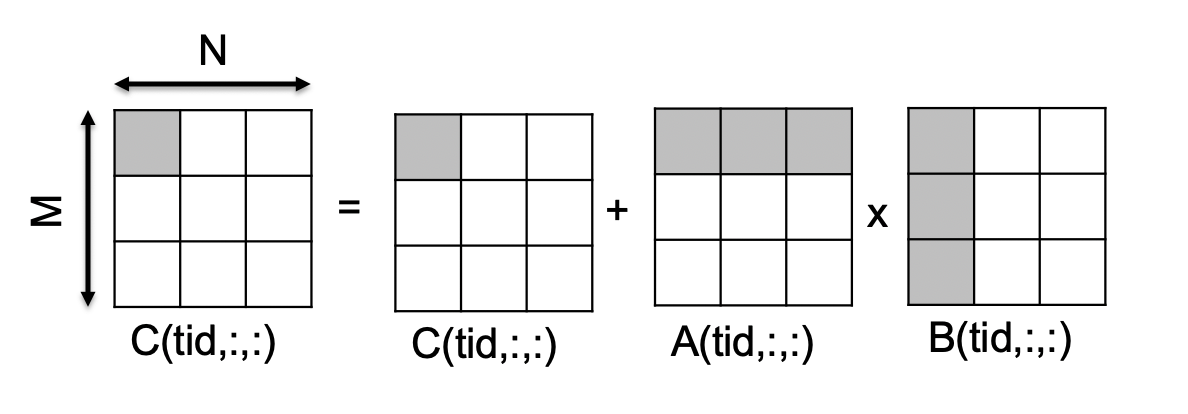
\includegraphics[width=0.65\textwidth]{figures/TeamGemm}
  \end{center}
\end{frame}

%==========================================================================
\begin{frame}[fragile]{KokkosBatched interfaces - TeamGemm}
  \begin{code}[keywords={parallel_for,auto,const,int}]
    Kokkos::parallel_for("teamGemmOuter", 
      Kokkos::TeamPolicy<ExecutionSpace>(nTeam, teamSize),
      KOKKOS_LAMBDA (const member_type &member) {
        const int tid = member.league_rank();
        // Each team performs a single TeamGemm
        Kokkos::parallel_for("teamGemmInner",
          Kokkos::TeamThreadRange(member, thisTeamsRangeSize),
          [=] (const unsigned int ij) {
            const int i = ij/N, j = ij%N;
            // each thread computes C(tid,i,j)
        });
    });
  \end{code}
  \vspace{10pt}
  \begin{center}
    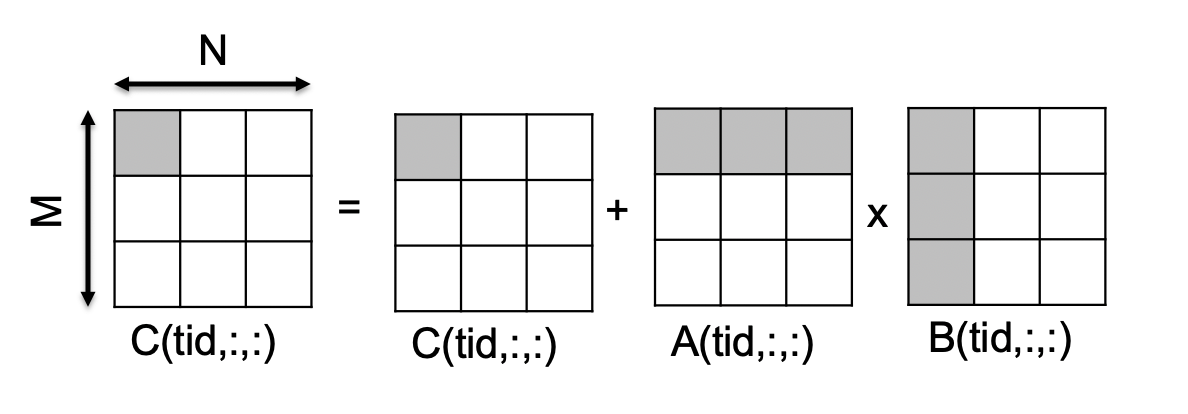
\includegraphics[width=0.65\textwidth]{figures/TeamGemm}
  \end{center}
\end{frame}

%==========================================================================
\begin{frame}[fragile]{KokkosBatched interfaces - TeamGemm}
  \textbf{This can be naturally expressed using the TeamGemm interface} \\
  \begin{code}[keywords={parallel_for,auto,const,int}]
    Kokkos::parallel_for("teamGemmOuter", 
      Kokkos::TeamPolicy<ExecutionSpace>(nTeams, teamSize),
      KOKKOS_LAMBDA (const member_type &member) {
        const int tid = member.league_rank();
        auto a = Kokkos::subview(A, tid, ALL(), ALL());
        auto b = Kokkos::subview(B, tid, ALL(), ALL());
        auto c = Kokkos::subview(C, tid, ALL(), ALL());
        KokkosBatched::TeamGemm(member, $\alpha$, a, b, $\beta$, c);
    });
  \end{code}
  \begin{center}
    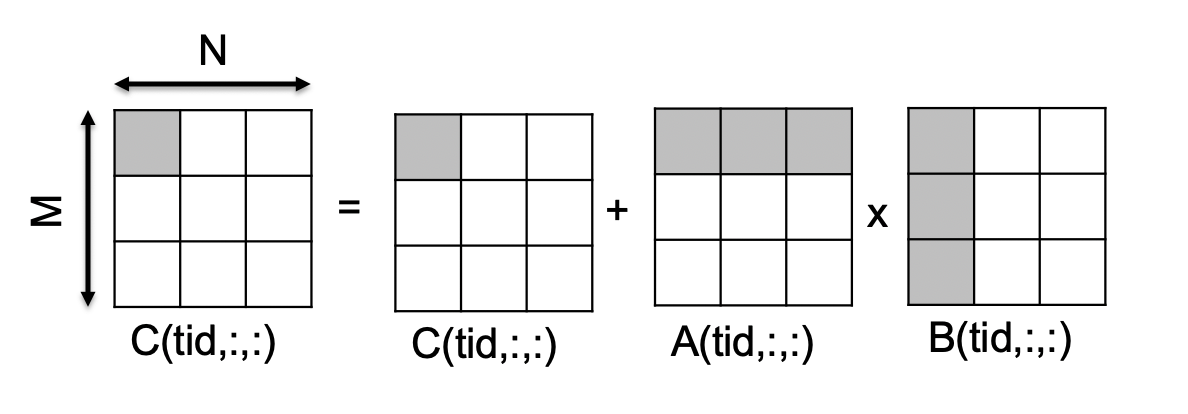
\includegraphics[width=0.65\textwidth]{figures/TeamGemm}
  \end{center}
  \vspace{-1em}
  \scriptsize{Related exercise available at: \verb!Exercises/kokkoskernels/TeamGemm!}
\end{frame}
%==========================================================================
\begin{frame}[fragile]{KokkosBatched interfaces - BlockJacobi}
  \Huge {Exercise: BlockJacobi}
\end{frame}

%==========================================================================
\begin{frame}[fragile]{KokkosBatched interfaces - BlockJacobi}

  \begin{itemize}
  \item Objective:
    \begin{itemize}
    \item \small{Compose a batched LU factorization of diagonal blocks and compute inverse of the blocks}
    \item \small{Compare a non-fused batched functions against the fused batch function using functor level interface} 
    \end{itemize}
  \item Exercise: \url{https://github.com/kokkos/kokkos-tutorials/tree/main/Exercises/kokkoskernels/BlockJacobi/Begin}
  \item On GPUs,
    \begin{itemize}
    \item Test the code with different team size \verb|run-different-teamsize.sh|
    \item Profile the code using nvprof \verb|run-nvprof.sh|
    \end{itemize}
  \end{itemize}

\end{frame}

%==========================================================================
\begin{frame}[fragile]{KokkosBatched interfaces - BlockJacobi}

  \begin{itemize}
  \item \small{\url{Exercises/kokkoskernels/BlockJacobi/Solution/run-different-teamsize.sh}}
  \item \small{This inverts 16,384 instances of 5x5 block matrices}
    \begin{tabular}{ccc}
      \hline
      \quad & \multicolumn{2}{c}{\# of inversion per sec} \\
      TeamSize & Non-fused & Fused \\
      \hline
      AUTO & 3,385 & \textbf<2>{5,054} \\
      32   & \textbf<3>{4,603} & \textbf<1,2,3>{8,766} \\
      64   & 4,199 & 6,488 \\
      96   & 3,581 & 5,017 \\
      \hline
    \end{tabular}
  \item Why 32 TeamSize is the best ?
    \begin{itemize}
    \item \footnotesize{For simplicity, assuming 25 entries of a block matrix are updated independently, 25 is the maximum team size}
    \item \footnotesize{By fusing multiple operations, temporal locality is exploited}
    \item \footnotesize{Need to check this using a profiler, nvprof}
    \end{itemize}
  \item \small{\url{Exercises/kokkoskernels/BlockJacobi/Solution/run-nvprof.sh}}
    \begin{itemize}
    \item<2-3> \only<2>{Comparison 1, AUTO vs 32} \only<3>{Comparison 2, non-fused vs fused}
    \end{itemize}
  \end{itemize}
  
\end{frame}

\begin{frame}[fragile]{KokkosBatched interfaces - BlockJacobi}

  Comparison 1: the same code with different team size
  \begin{itemize}
  \item \footnotesize{AUTO (set TeamSize = 96) shows higher occupancy}
    \begin{center}
      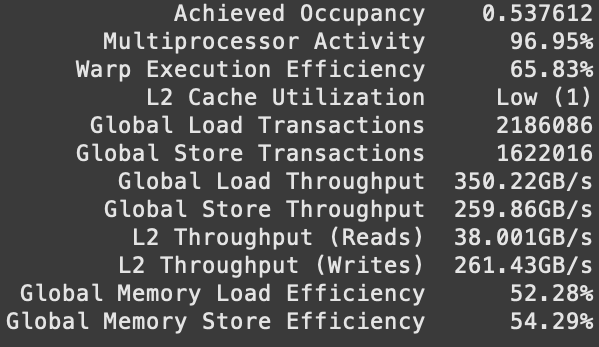
\includegraphics[width=0.40\textwidth]{figures/BATCHED-blockjacobi-auto-fused.png}
    \end{center}
  \item \footnotesize{TeamSize = 32 leads higher global load/store throughput, resulting 1.7x speedup }
    \begin{center}
      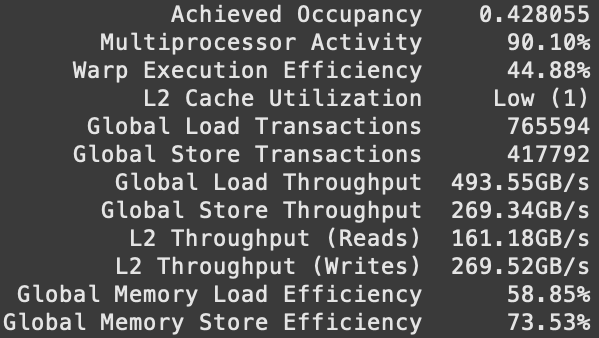
\includegraphics[width=0.40\textwidth]{figures/BATCHED-blockjacobi-team32-fused.png}
    \end{center}
  \end{itemize}

\end{frame}

\begin{frame}[fragile]{KokkosBatched interfaces - BlockJacobi}

  Comparison 2: the same code with non-fused vs fused version
  \begin{itemize}
  \item \footnotesize{For non-fused version, we show one best performing kernel of four kernels}
    \begin{center}
      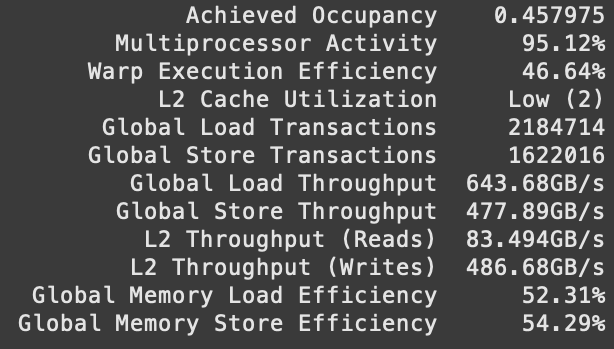
\includegraphics[width=0.40\textwidth]{figures/BATCHED-blockjacobi-team32-nonfused.png}
    \end{center}
  \item \footnotesize{Fused version performs 1.9x faster than non-fused version}
    \begin{center}
      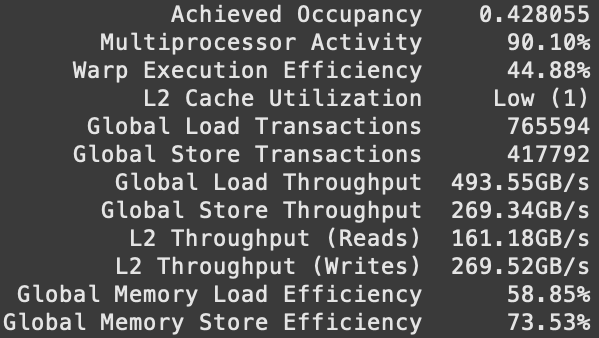
\includegraphics[width=0.40\textwidth]{figures/BATCHED-blockjacobi-team32-fused.png}
    \end{center}
  \item \footnotesize{Note that non-fused interface can be optimized much better for each kernel and specific problem size}
  \end{itemize}

\end{frame}

\begin{frame}[fragile]{Summary}

  \textbf{Summary: Batched BLAS/LAPACK}
  \begin{itemize}
  \item \small{User composable batched interface: parallel execution policy + functor-level interface}
  \item \small{Performance on GPUs is tunable:}
    \begin{itemize}
    \item \small{Launching light-weight kernels multiple times can cause overhead}
    \item \small{Fusing too many functor-level BLAS/LAPACK operations is difficult to perform optimal with a single team size}
    \end{itemize}
  \end{itemize}
  
\end{frame}
